\documentclass[11pt]{beamer}

%=================================================
% theme and color
%=================================================
\usetheme{Warsaw} %Themes http://www.hartwork.org/beamer-theme-matrix/
\definecolor{colorA}{RGB}{0, 140, 200}
\definecolor{colorB}{RGB}{140, 151, 154}
%\definecolor{secinhead}{RGB}{249,196,95}
%\definecolor{titlebg}{RGB}{51,51,51}
\setbeamercolor{structure}{fg=colorA,bg=colorB}
%\setbeamercolor{secsubsec}{fg=secinhead,bg=black}
%\setbeamercolor{frametitle}{fg=secinhead,bg=titlebg}

%=================================================
% packages and new commands
%=================================================
\usepackage{xcolor}
\usepackage[ruled, linesnumbered, vlined]{algorithm2e}
\usepackage{epsfig, subfigure, amssymb, multirow, algorithmic, amsmath}
\newcommand*{\superscript}[1]{\ensuremath{^{\rm #1}}}
\newcommand*{\subscript}[1]{\ensuremath{_{\rm #1}}}

%=================================================

\newenvironment<>{proposition}[1][\undefined]{%
\begin{actionenv}#2%
\ifx#1\undefined%
   \def\insertblocktitle{Proposition}%
\else%
   \def\insertblocktitle{Proposition ({\em#1})}%
\fi%
\par%
\mode<presentation>{%
%  \setbeamercolor{block title}{fg=white,bg=yellow!50!black}
%  \setbeamercolor{block body}{fg=black,bg=yellow!20}
}%
\usebeamertemplate{block begin}\em}
{\par\usebeamertemplate{block end}\end{actionenv}}



\AtBeginSection[]{
  \begin{frame}
  \vfill
  \centering
  \begin{beamercolorbox}[sep=8pt,center,shadow=true,rounded=true]{title}
    \usebeamerfont{title}\insertsectionhead\par%
  \end{beamercolorbox}
  \vfill
  \end{frame}
}

% thesis details (preamble)
%=================================================
\title[{\sc  } \hspace{0.8cm} \insertframenumber/\inserttotalframenumber]{{\sc Simgrid as a platform }}
\author[Myriads - ADT]{{Toufik Boubehziz}}%--- {\sc Feb 10\superscript{th}, 2015}
\date{September 28, 2017}
\institute{INRIA - Bretagne Atlantique}

%=================================================
% start presentation
%=================================================
\begin{document}

%========================


% title page
%========================
\begin{frame}
\maketitle
\begin{center}

\includegraphics[width=3.5cm]{figures/inria.png}
\end{center}
\end{frame}

%========================
% your slides:
%========================
\section{Overview of SimGrid APIs}
\begin{frame}
SimGrid is a simulator project that provides core toolkit for the simulation of distributed applications in heterogeneous distributed environments.\\
\begin{figure}
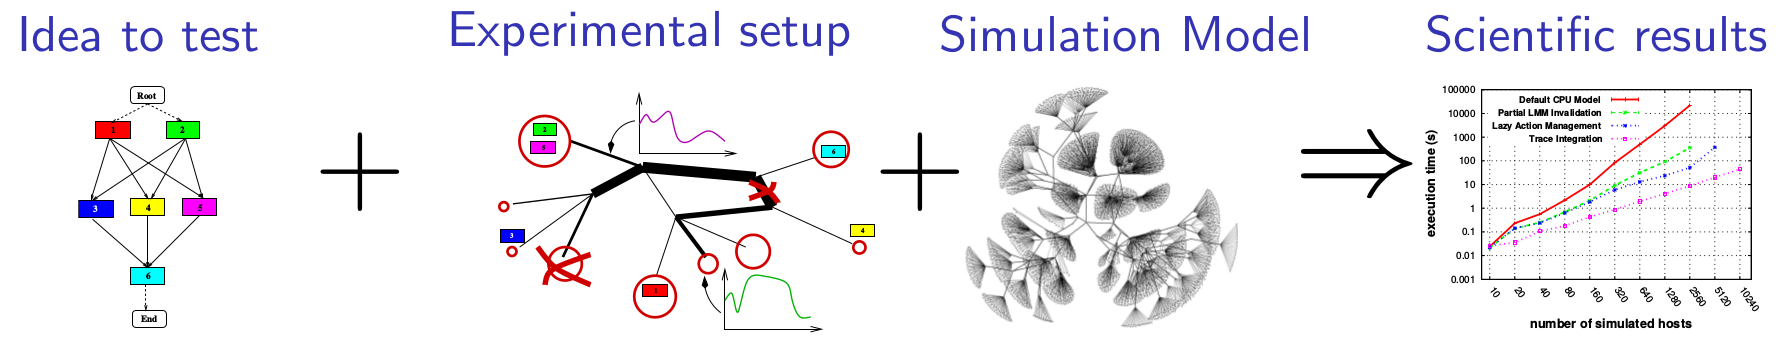
\includegraphics[width=11cm]{figures/simgrid.png}
\end{figure}
The aim goal of the project is to give an efficient tool for research in the area distributed large scale systems, like as Grids, P2P systems and Cloud.
\end{frame}

\begin{frame}
\tableofcontents
\end{frame}


\begin{frame}\frametitle{An overview of SimGrid}

\begin{figure}
  \begin{center}
    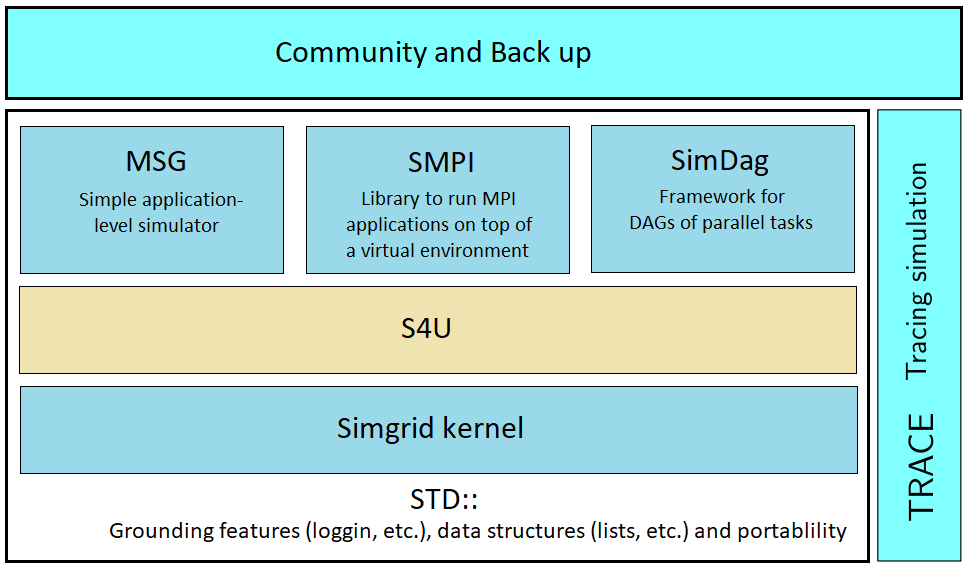
\includegraphics[width=10cm]{figures/simgridplan1.png}
  \end{center}
\end{figure}
\end{frame}

%========================
% example slides:
%========================
\section{Tracing simulation}
\begin{frame}\frametitle{Tracing simulation}
Simgrid despose of a visualization tracing model that works through gathering data about the resource of links and hosts of a turned simulation whatever the interface (MSG, SimDag, SMPI, and S4U).\\

%The idea of the tracing facilities is to give SimGrid users to possibility to classify MSG and SimDAG tasks by category. \\
\begin{exampleblock}{Tracing before}
The previous model was written under C code in such way it emulate the CPP OOP.
\end{exampleblock}
%This latter mean that any task is not classified according to a category is not traced. If no categories are specified, simulations can still be traced using a special parameter in the command line.

%This means that the tracing will register how much power is used for each host and how much bandwidth is used for each link of the platform.
\end{frame}
\begin{frame}\frametitle{Tracing after}
\begin{exampleblock}{}
We were able to make some several improvements on the code 
\begin{itemize}
\item Remove the useless structures and functions.
\item Make an hierarchical class tree that are shown in the below figure.
\end{itemize}
\end{exampleblock}
\begin{figure}
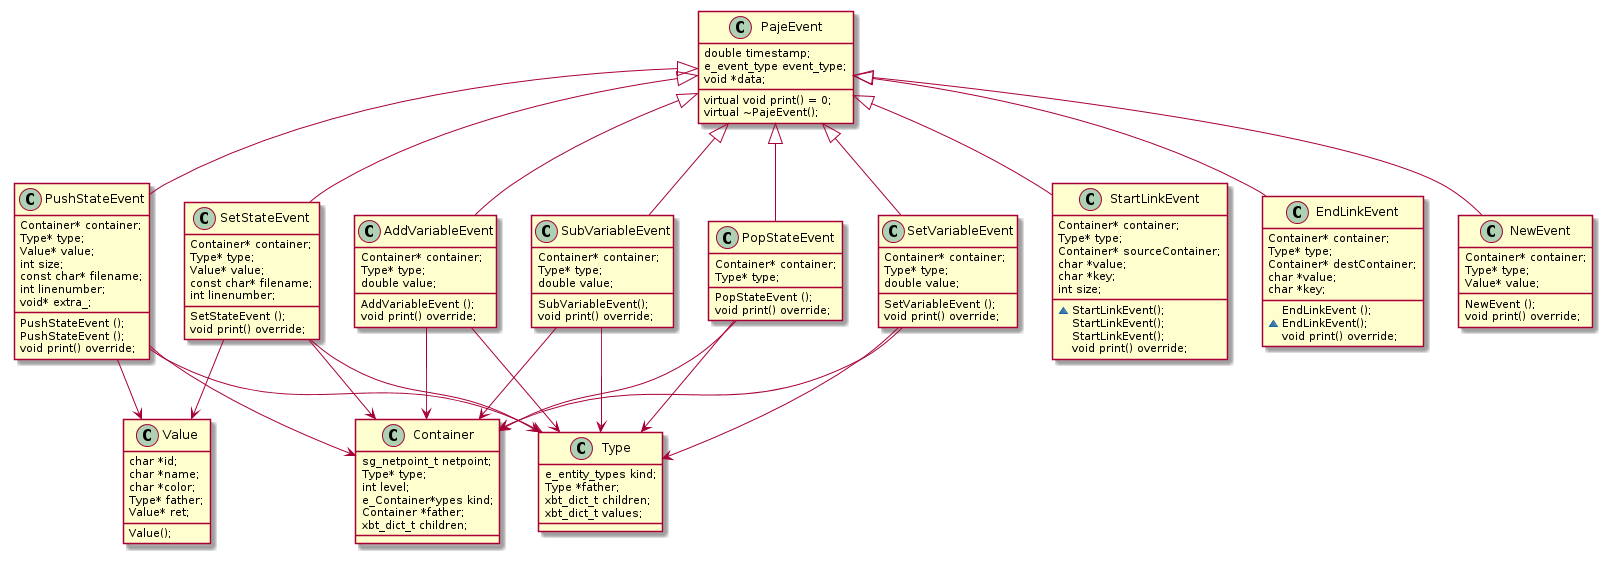
\includegraphics[width=10.5cm]{figures/diagram_simgrid.png}
\end{figure}
\end{frame}
%------------------------
\section{S4U interface}
\begin{frame}%\frametitle{S4U plateforme}
\begin{block}{}
S4U is the new core API under \textsf{C++} that will eventually replace MSG and SimDag APIs. In other word, Everything that could be done in SimGrid will be possible in S4U.
\end{block}
%Currently, we are interested by given to S4U users a similar models as MSG, in order to give them an punsh of examples that could be used and modified as desired.  

\begin{figure}
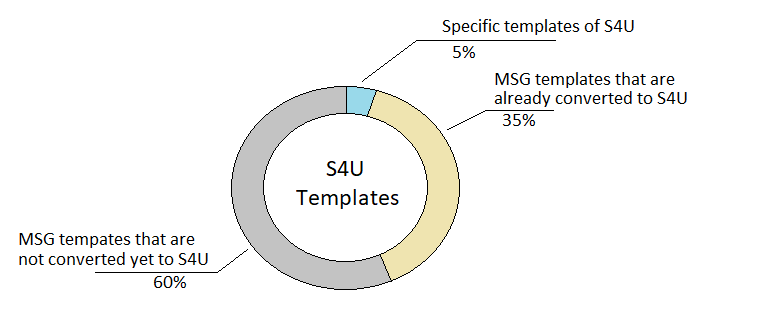
\includegraphics[width=10cm]{figures/s4ud.png}
\end{figure}
\end{frame}
%------------------------
\section{Simgrid numerical support}
\begin{frame}
SimGrid has a tutorial support that is always updated and a practical course via it platform SimGrid Courseware. %This latter is targeting academic community that want to learn MPI.
% by give to them an interesting models to solve.
\begin{block}{}
\begin{itemize}
\item Check and report any abnomality could be found in tutorial support of simgrid \href{http://simgrid.gforge.inria.fr/}{\beamergotobutton{http://simgrid.gforge.inria.fr/}}.\\
\item Check the courseware tools compatibility with the new version of simgrid 3.16 \href{https://simgrid.github.io/SMPI\_CourseWare/}{\beamergotobutton{https://simgrid.github.io/SMPI\_CourseWare/}}.   
\end{itemize}
\end{block}
\end{frame}
%----------------------------------------------------------------

%Get them from
%http://simgrid.gforge.inria.fr/documentation.html
%\begin{block}{}
%\begin{itemize}
%\item Practical introduction to SimGrid and MSG
%\item Platforms and experiments in SimGrid
%\item Practical introduction to the use of SimDag
%\item Visualization of SimGrid simulation results
%\item Simulation MPI applications in practice
%\item Model-checking of SimGrid programs
%\item The Platform Models underlying SimGrid
%\item Kernel of SimGrid
%\end{itemize}
%\end{block}
%------------------------
\section{Community and backup}
%\subsection{Bugs tracking}
\begin{frame}\frametitle{Bugs tracking and community of simgrid}
There are few several ways that we use to support the community, improve continuously simgrid, and interact with the other members.
\begin{enumerate}
\item Follow the mailing lists to be aware about the issues that face the community \textcolor{blue}{\url{simgrid-user@lists.gforge.inria.fr}}. 
\item Participate in discussions on \textcolor{blue}{IRC} channel \textcolor{blue}{$\# $simgrid} on \textcolor{blue}{oftc} servers. %The channel allowed to having exchange of ideas, resolve issues efficiently and having back up if one is in trouble. 
\item Attend scheduled meetings by project members to get an idea of the different parts of the code.
\item Participate to the bug tracking via \textcolor{blue}{Github issues} and \textcolor{blue}{Sonar}.
\end{enumerate}
\end{frame}
\begin{frame}\frametitle{Workflow}
\begin{figure}
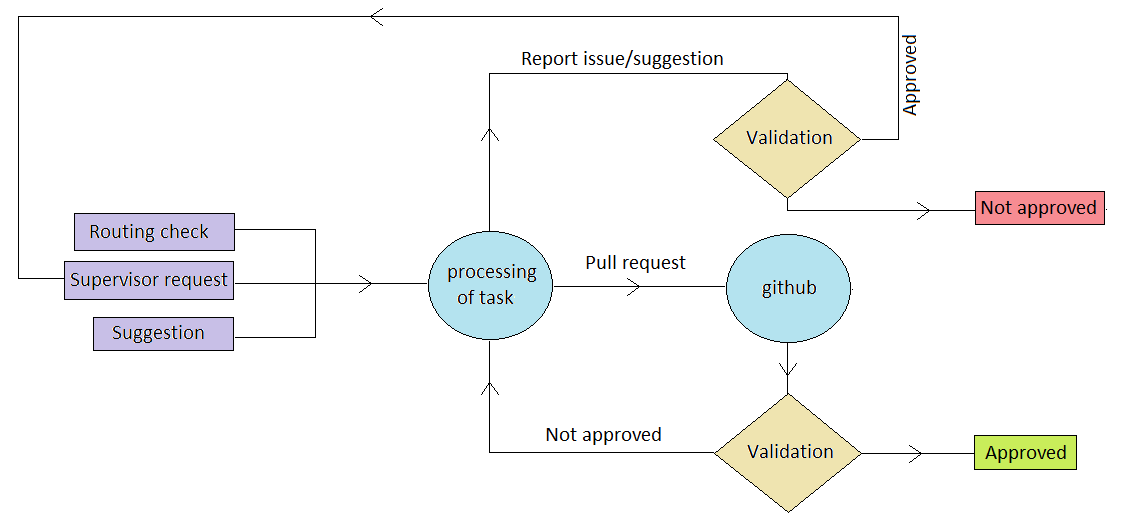
\includegraphics[width=11cm]{figures/productiont.png}
\end{figure}
\end{frame}
\begin{frame}\frametitle{Validation tools}
SimGrid dispose of a bunch of testing procedures that are used to detect bugs and bad written of code.
\begin{itemize}
\item \textcolor{blue}{Jenkins} : a self-contained automation server which allowed to automate any kind of tasks related to building, testing, and deploying software.
\item \textcolor{blue}{Travis-ci} : a hosted, distributed continuous integration service used to build and test software projects hosted at GitHub.
\item \textcolor{blue}{Codacy} : an automated code review application that includes static analysis functionality.
\item \textcolor{blue}{SonarQube} : an open source platform for inspect the code quality with static analysis of code.
\end{itemize}

\end{frame}
%------------------------

%------------------------
\section{Perspectives}
\begin{frame}\frametitle{Perspectives}
In the further time, we plan to : 
\begin{itemize}
\item Complete the s4u platforme.
\item Write a tutorial for S4U.
\item Continue the refactoring of the kernel simgrid .
%\item Add a scriptable models (by using Lua language).
\item Collect and classify templates, examples and contributions.
\item Launch an efficient forum for users.
\item Community animation.
\end{itemize}
\end{frame}
%========================
% bibliography
%========================
%\input{slides/bib}

%=================================================
% end presentation
%=================================================
\end{document}